%
% Copyright (c) 2008 Betti "Osterholz
%
% Permission is granted to copy, distribute and/or modify this document
% under the terms of the GNU Free Documentation License, Version 1.2 or
% any later version published by the Free Software Foundation;
% with no Invariant Sections, no Front-Cover Texts, and no Back-Cover Texts.
%
% A copy of the license is included in the file ``fdl.tex'' .
%

%path for pictures
\graphicspath{{./material_enviroment/}}
\graphicspath{{./material_enviroment/}{../material_enviroment}}

\newpage
\part{Der genetische Algorithmus}\index{genetischer Algorithmus}\index{Algorithmus}
\label{secGeneticAlgorithmDesign}

In diesem Abschnitt werden allgemeine Entwurfsentscheidungen und erste Analysen f"ur den genetischen Algorithmus aufgestellt.
Der realisierte genetische Algorithmus ist flexibel und erweiterbar gestaltet.

Der genetische Algorithmus ist nat"urlich auch ein evolution"arer Algorithmus. Die Bezeichnung ``genetisch'' bezieht sich auf die F"ahigkeit des Algorithmus, Informationen von zwei oder mehr Individuen in einem neuen Individuum zu kodieren und darauf, dass er auf Informationen arbeitet, die ein (Multimedia-) Objekt kodieren und diese Objekte nicht direkt darstellen.

Der Algorithmus dient zur Erzeugung/Generierung von Fib-Objekten, welche ein Multimediaobjekt m"oglichst gut darstellen. Dem Algorithmus wird daf"ur ein bestimmtes Multimediaobjekt vorgegeben, f"ur dass er Fib-Objekte/Individuen generiert, von denen gute selektiert werden. Die Generierung von Individuen kann auch Analysen des Multimediaobjekts beinhalten und die Nutzung oder Analyse von Informationen anderer Individuen. Welche Individuen gut sind, wird mithilfe von vorgegebenen Parametern entschieden (durch den Bewerter f"ur Individuen).

\bigskip\noindent
Der Algorithmus besteht aus f"unf separaten Teilen:
\begin{itemize}
 \item dem Kernalgorithmus
 \item dem Bewerter f"ur Individuen
 \item dem Mortalit"atsbewerter
 \item dem Bewerter f"ur Operatoren
 \item der Menge der Operatoren
\end{itemize}

In der Abbildung \ref{figGeneticAlgorithmus} ist eine Ablaufskizze des genetischen Algorithmus dargestellt.

\begin{figure}[htbp]
\begin{center}
  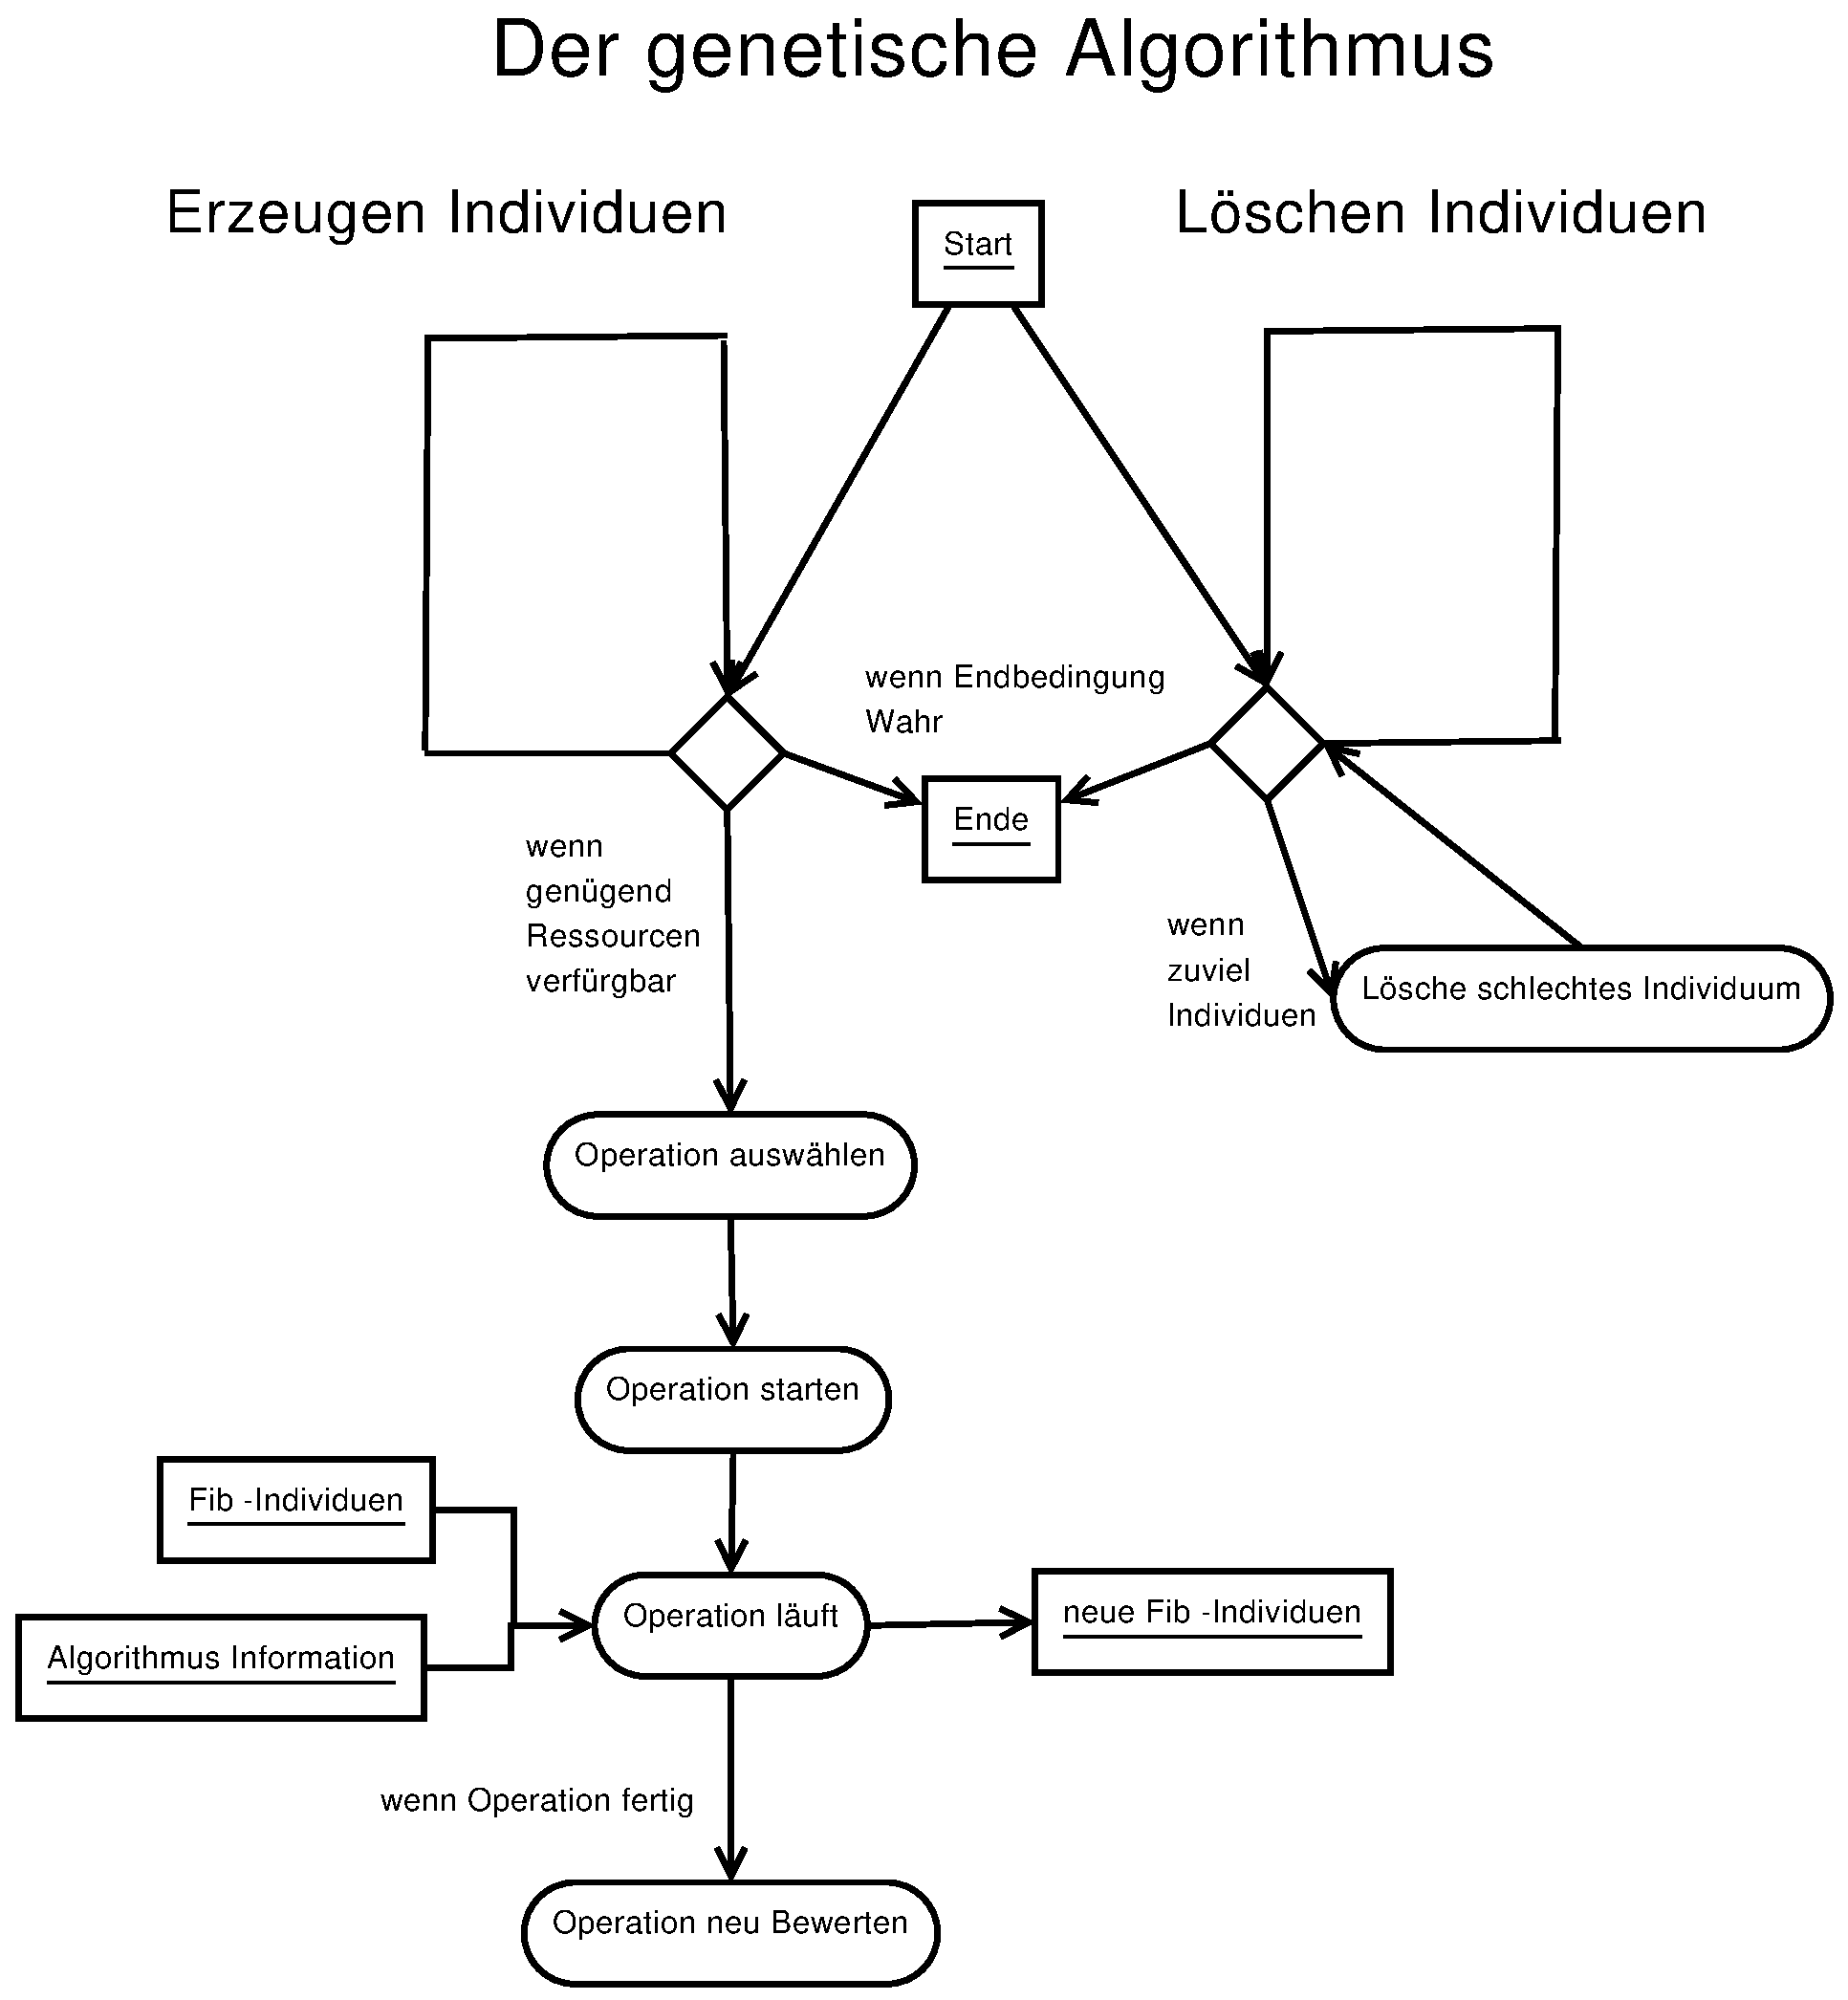
\includegraphics[scale=0.4]{algorithmus}
\end{center}
\caption{Ablaufskizze des genetischen Algorithmus}
\label{figGeneticAlgorithmus}
\end{figure}


Im Nachfolgenden werden die einzelnen Fib-Objekte als Individuen bezeichnet. Die Menge aller Individuen, die zu einem Zeitpunkt im Algorithmus vorhanden sind, wird kurz als Population bezeichnet.


\section{Kernalgorithmus}\index{Kernalgorithmus}

Der Kernalgorithmus nutzt die Bewerter und die Operatoren, um den genetischen Algorithmus zu realisieren. Er soll m"oglichst einfach gehalten und flexibel sein.

Die Bewerter f"ur Individuen oder Operatoren sind ("uber Parameter) austauschbar.

\bigskip
Der Kernalgorithmus beinhaltet einmal die Hauptschleife des genetischen Algorithmus, in dem die Operatoren aufgerufen und Individuen erzeugt werden.

Als zweite Schleife existiert im Algorithmus die Selektionsschleife. Durch sie werden Individuen gel"oscht.

\bigskip
Des Weiteren stellt der Kernalgorithmus Funktionen f"ur die Operatoren bereit. Die Operatoren werden vom Kernalgorithmus "uber eine Methode aufgerufen, die f"ur alle Operatoren gleich ist. Danach holen sich die Operatoren "uber Funktionen des Kernalgorithmus spezifische Werte aus dem Algorithmus, wie z. B. die Individuen, auf denen die Operationen arbeiten. Auf diese Weise sehen die Operatoren f"ur den Kernalgorithmus immer jeweils gleich aus, und er ben"otigt keine Logik speziell f"ur einen bestimmten Operator. Damit werden auch zuk"unftige Anpassungen der Operatoren vereinfacht, da nicht die Schnittstelle aller Operatoren angepasst werden muss, sondern nur die Funktionen, welche der Kernalgorithmus bereitstellt.

Die Aufrufmethode f"ur die Operatoren soll flexibel sein, so dass auch Operatoren nebenl"aufig gestartet werden k"onnen und nicht auf die Beendigung jedes Operatoraufrufs gewartet werden muss. Die Operatoren sollten getrennt vom Kernalgorithmus laufen und diesen nur "uber die vorgegebene Schnittstelle beeinflussen k"onnen. Ein fehlerhafter Operator soll also nicht zu Fehlern im oder zur Beendigung des Gesamtsystems f"uhren.


\section{Bewerten von Individuen}\index{Bewerter!Individuen}\index{Individual!Bewerter}

Der konkrete Bewertungsalgorithmus sollte einfach auszutauschen sein, um verschiedenen Problemstellungen Rechnung tragen zu k"onnen. Der jeweilige Bewertungsalgorithmus wird zur Berechnung der Fitness eines Individuums ben"otigt.

"Uber Parameter f"ur spezielle Bewerter k"onnen diese weiter angepasst werden (beispielsweise damit eingestellt werden kann, wie wichtig eine geringe Gr"o"se gegen"uber eine schnellen Auswertung von Individuen ist).


\subsection{Die Fitness eines Individuums}\index{Fitness!Individuen}\index{Individual!Fitness}

Die Fitness eines Individuums ist durch verschiedene Fitnessfaktoren gegeben.

Einer der wichtigsten ist, inwieweit das Individuum den gew"unschten Originalmultimediadaten (z. B. dem Originalbild) "ahnelt. Je mehr das Individuum (bzw. der Ph"anotyp dessen) den Originalmultimediadaten "ahnelt, umso h"oher sollte die Fitness sein und umso geringer ist der Fehler, den das Individuum f"ur die Darstellung der Originalmultimediadaten macht.

Dieser Fehler (und damit die Fitness des Individuums) kann z. B. "uber die Summe der (quadratischen) Abweichungen (nicht definierte Punkte liefern einen maximalen Fehler) in den Farben zu einem Punkt zwischen dem Originalbild und dem vom Individuum erzeugten Bild bestimmt werden oder "uber ein anderes selbstbestimmtes Abstandsma"s.

Wenn die Fitness f"ur einzelne Teilobjekte des Individuums bestimmt wird, kann dies z. B. dadurch realisiert werden, dass in die Rechnung nur der Bereich einbezogen wird, der durch das Teilobjekt "uberdeckt wird, ein Rand um diesen Bereich noch mit einbezogen wird, oder auch nur das kleinste Quadrat benutzt wird, das dieses Objekt umschlie"st.

Ein anderer sinnvoller Fitnessfaktor ist die Gr"o"se (steigt mit der Anzahl der Elemente) der einzelnen Individuen, um gr"o"seren Individuen eine geringere Fitness zu geben als kleineren Individuen, mit dem gleichen Fehler auf den Originalmultimediadaten, und die kleineren Individuen so zu bevorzugen.

Ein weiterer Fitnessfaktor der einbezogen werden kann, ist eine Sch"atzung "uber die Zeit, die f"ur das Individuum zur Berechnung des dargestellten Multimediaobjekts (Ph"anotyp) ben"otigt wird. Damit kann eventuell sogar die Ausf"uhrungsgeschwindigkeit des Algorithmus erh"oht werden.


\subsection{Selektion durch L"oschen von Individuen}\index{Selektion}

Um die Ressourcen (Arbeitspeicher, Rechenzeit) zu schonen, ist es notwendig, die Anzahl der Individuen (Fib-Objekte) im Bearbeitungsprozess (Individuen die noch am genetischen Algorithmus teilnehmen) zu beschr"anken. Deshalb m"ussen Individuen aus diesem (nach Bedarf) entfernt werden. Dabei sind Individuen mit einer niedrigen Fitness zu bevorzugen.

Deshalb gibt es f"ur den Algorithmus einen \textbf{Mortalit"atsbewerter}\index{Mortalit"atsbewerter}. Dieser bestimmt, mit welcher Wahrscheinlichkeit ein Individuen gel"oscht wird. Um Individuen zu l"oschen, gibt es im Algorithmus eine seperate Schleife, in der gepr"uft wird, ob die maximale Anzahl von Individuen "uberschritten ist. Wenn dies der Fall ist, werden so viele Individuen gel"oscht, bis die maximale Anzahl von Individuen wieder eingehalten wird. Dabei haben Individuen mit einer hohen Bewertung durch den Mortalit"atsbewerter auch eine hohe Wahrscheinlichkeit, gel"oscht zu werden.

Der Mortalit"atsbewerter orientiert sich f"ur seine Bewertung an der Fitness der Individuen. Er kann allerdings durch andere Mortalit"atsbewerter ausgetauscht oder durch Parameter gesteuert werden. Es ist beispielsweise auch m"oglich, einige Individuen als unsterblich bzw. nicht l"oschbar zu deklarieren. Indem z. B. die $n$ ($n>0$) besten Individuen als unsterblich deklariert werden, kann vermieden werden, dass diese gel"oscht werden und somit eines der besten Individuen verloren geht.

Der Mortalit"atsbewerter kann weiterhin "uber die Operatorschnittstelle auf Statusinformationen des Algorithmus zugreifen, um z. B. die Anzahl der bisher erzeugten Individuen zu ermitteln.


\section{Bewerter f"ur Operatoren}\index{Bewerter!Operatoren}

Um zu bestimmen, welcher Operator als n"achstes ausgew"ahlt wird, sind diese zu bewerten. Operatoren, die besser in einer Situation bewertet werden, haben eine h"ohere Wahrscheinlichkeit, in einer "ahnlichen Situation ausgew"ahlt bzw. ausgef"uhrt zu werden.

\bigskip\noindent
Die Situation kann umfassen:
\begin{itemize}
 \item die wievielte Operation bzw. Interaktion ausgef"uhrt wird.
 \item welcher Art das Originalmultimediaobjekt ist ("uber die Definitionen f"ur die Umgebung in den root-Elementen dieses):
 \begin{itemize}
  \item es enth"alt Farben 
  \item es ist Schwarz/Wei"s
  \item es enth"alt Ton
  \item es handelt sich um einen Film
  \item ...
 \end{itemize}
 \item die durchschnittliche (relative) Fitness der Individuen.
 \item die Fitness des besten/schlechtesten Individuums.
 \item die Standardabweichung der Fitnesswerte in der Population.
 \item die Anzahl der Individuen.
 \item Operationen, die bisher angewendet wurden.
 \item ...
\end{itemize}

Der spezielle Bewertungsalgorithmus kann ausgew"ahlt werden. So k"onnen verschiedene Bewertungsalgorithmen leicht gegeneinander ausgetauscht und verglichen werden.

Zur Bewertung der Operatoren werden (von einzelnen Bewertern) eventuell Daten "uber ihre bisherigen Anwendungen permanent gehalten. Auf diese Weise kann der Algorithmus aus vorhergehenden Operatoraufrufen lernen.

Die Bewertung der Operatoren sollte m"oglichst Systemunabh"angig erfolgen, also unabh"angig vom Rechner, auf dem der Algorithmus gerade l"auft.

\bigskip\noindent
Die Bewertungskriterien k"onnen sein:
\begin{itemize}
 \item Ausf"uhrungszeit der Operation
 \item erreichte Verschlechterungen oder Verbesserungen
 \item Zuverl"assigkeit des Operators (Gibt er immer ein Ergebnis zur"uck? St"urzt er manchmal ab?)
 \item ...
\end{itemize}


\section{Die genetischen Operationen auf Fib}

Die Operatoren sind vom genetischen Algorithmus getrennt zu sehen. Es sollte m"oglich sein, beliebig viele Operatoren zum genetischen Algorithmus hinzuzuf"ugen, ohne diesen anpassen zu m"ussen.

Jeder Operator hat eine eindeutige Kennung bzw. ID, "uber die ihm zugeh"orige Werte (z. B. seine bisherige Performance) zugeordnet werden k"onnen.

Wird ein Operator ausgef"uhrt, ist dies eine Operation.

Diese Operationen sind dazu gedacht, Kodierungsalgorithmen zu implementieren. Operatoren sollten also nicht m"oglichst einfach sein, sondern k"onnen durchaus komplexe Algorithmen beinhalten.

Die Operatoren sollen auch m"oglichst zahlhaft sein, und der Algorithmus ist f"ur die Auswahl guter Operatoren verantwortlich. Daher ist es auch erw"unscht, mit sinvollen Teilen von Operatoren eigene Operatoren zu erstellen. Dabei sollten sowohl die Originaloperatoren als auch der Operator, der den extrahierten Teil enth"alt, im Algorithmus verbleiben.

F"ur Spezialanwendungen kann ein genetischer Algorithmus verwendet werden, dessen Menge der Operatoren auf die n"utzlichsten f"ur diese Anwendung eingeschr"ankt wurde.
Auch k"onnen f"ur eine Anwendung n"utzliche Operatoren zu einem (nicht genetischen) Algorithmus kombinert werden, der diese in determinerter Weise verbindet.


\subsection{Vermehrung}

Bei der ``Vermehrung'' wird im Allgemeinen ein Individuum aus der Population genommen, bevorzugt Individuen mit hoher Fitness, dieses kopiert und durch eine Operation ver"andert. Ist das entstehende Individuum ein ``neues'' Objekt (wenn es kein gleiches in der Population gibt), wird es zur Menge hinzugenommen. Es k"onnen auch bereits vorhandene Individuen "ubernommen werden.

Im Algorithmus wird die Vermehrung dadurch realisiert, dass eine Operation ausgef"uhrt wird. Diese Operation holt sich dann "uber die Operationenschnittstelle vom Algorithmus alle ben"otigten Daten. Zu den ben"otigten Daten k"onnen ein oder mehrere Individuen geh"oren oder Daten "uber den bisherigen Verlauf des Algorithmus (z. B. die Nummer der bisherigen Interaktionen bzw. Operationen).


\section{Der soziale Aspekt des genetische Algorithmus}\index{Algorithmus!Sozialkomponente}

Die strikte Trennung der Operatoren vom Algorithmus und die M"oglichkeit, Operationen leicht hinzuf"ugen zu k"onnen, hat seinen Grund in eher sozialen "Uberlegungen.

Normale Kodierungsalgorithmen beschr"anken sich bei den Kodierungsmethoden auf eine oder nur wenige Ideen von einigen (in der Gr"o"senordnung von 1 bis 100) Menschen (dem Entwicklerteam). Da es aber viel mehr (in der Gr"o"senordnung von wahrscheinlich 100000) Menschen weltweit gibt, die sich im weiteren Sinne mit der effizenten Kodierung von Multimediaobjekten besch"aftigen, bleiben dadurch zwangsl"aufig auch viele Ideen zur Kodierung unber"ucksichtigt. Selbst wenn ein Teil dieser Menschen daran Interesse hat, ihre Ideen einzubringen, ist dies nur sehr schwer bis unm"oglich zu realisieren.

In den Fib-Algorithmus kann aber jeder neue Ideen in Form neuer Operatoren einbringen (ein Begriff daf"ur ist ``Crowdsourcing''). Daf"ur sind lediglich ausreichende Kenntnisse der Fib-Multi\-media\-beschrei\-bungs\-sprache und der Schnittstelle des Algorithmus f"ur die Operatoren n"otig. Um neue Ideen bzw. Operatoren zur effizenten Kodierung von Multimediaobjekten einzubringen, sollten keine Anpassungen am Algorithmus oder anderen Operatoren n"otig sein. Dadurch werden Seiteneffekte beschr"ankt und jede Implementierung einer Idee hat sich nur um die Idee bzw. deren Operator zu k"ummern. Es sind also keine weiteren Kenntnisse des Algorithmus oder gar anderer Operatoren von N"oten. Auf diese Weise kann das System wachsen, ohne dass sich die Komplexit"at des (Kern-)Systems vergr"o"sert und die Wartung und Erweiterung des Systems schwieriger wird.

Der Algorithmus und die Bildbeschreibungssprache sollten so angelegt sein, dass sich auch Laien ohne gr"o"seren Aufwand einarbeiten und neue Ideen bzw. Operatoren realisieren k"onnen. Insbesondere sollten Studenten und Studierende (z. B. Menschen mit Informatik als Hobby) der Informatik, sich innerhalb weniger Tage soweit einarbeiten k"onnen, dass sie einen eigenen Operator realisieren und einbinden k"onnen. (Wie n"utzlich oder effizient dieser ist, sei erst einmal dahingestellt.)

Die GNU-GPL-Lizenz, unter dem der Algorithmus steht, kl"art die rechtliche Situation, unter der neue Operatoren stehen. Dadurch k"onnen neue Operatoren legal eingebunden werden, solange nicht andere Rechte verletzt werden (eine Verletzung w"are beispielsweise, dass in den Operatoren verwendete Algorithmen oder Codes unter inkompatiblen Lizenzen stehen). Neue Operatoren k"onnen auch der Allgemeinheit zur Verf"ugung gestellt werden.

Die Bewertung der Operatoren sollte motivieren, eigene Operatoren einzubinden. Dadurch kann jeder, der einen Operator hinzugef"ugt hat, realistisch einsch"atzen, wie gut sein Operator sich im Verh"altnis zu anderen Operatoren in einer Situation macht. Der Wettbewerb unter Operatorenautoren sollte f"ur neue bessere Operatoren f"orderlich sein.


All dies sollte dazu f"uhren, dass nicht nur ein kleines Entwicklerteam zur Verbesserung der Kodierung von Fib-Objekten beitr"agt, sondern dass ein viel gr"o"serer Kreis von Menschen sich mit diesen Thema besch"aftigt. Dies sollte der Entwicklung und Verbreitung von Fib einen weiteren Schub geben.

In diesem Sinne ist der genetische Algorithmus f"ur Fib ein transgenialer Algorithmus, der darauf angelegt ist, die Ideen von Menschen zur Kodierung von Multimediadaten aus deren K"opfen herauszuholen und in einem Topf zu transportieren/sammeln. Damit sollen diese Ideen/Algorithmen mehr leisten k"onnen, als sie es einzeln k"onnten. Der Algorithmus kann damit mehr Intelligenz in sich vereinen, als es ein Mensch (oder auch eine kleine Gruppe) hervorbringen kann.


\section{Warum sich genetische Algorithmen zur Multimediakodierung anbieten}

Es gibt im Allgemeinen keinen Algorithmus der Rastergrafiken direkt in speicherschonende Vektorbilder umwandeln kann, bei denen die St"arken der entsprechenden Vektorbeschreibungssprache wirklich genutzt werden. F"ur die Umwandlung von einem Multimediaformat in ein anderes ergibt sich oft eine "ahnliche Problematik, insbesondere wenn das erste Multimediaformat die Eigenschaften von Punkten eines euklidischen (diskreten) Raumes direkt angibt (z. B. um Aufnahmen direkt abspeichern zu k"onnen) und das zweite Multimediaformat komplexe Objekte (z. B. Rechtecke oder/und Kreise) in Multimediaobjekten kodiert.

Da ein genetischer Algorithmus das Potential hat, alle m"oglichen Beschreibungen einer Multimediasprache zu generieren und unter diesen nat"urlich auch gute Beschreibungen sind, welche die St"arken der Multimediasprache in Bezug auf das Originalobjekt nutzen, hat ein genetischer Algorithmus nat"urlich auch das Potential, gute Beschreibungen zu generieren. Wenn im genetischen Algorithmus vorhandenes Wissen gut eingebaut wurde, kann er gute Beschreibungen wahrscheinlich auch schneller finden als eine reine Zufallssuche.

Noch ein weiterer Vorteil von genetischen Algorithmen ist die gro"se Freiheit bei der Wahl der Problembeschreibung (Multimediasprache) und der m"oglichen Operatoren auf dieser. So kann v"ollig frei eine Multimediasprache nach eigenen Vorstellungen entworfen werden, die bestimmte Eigenschaften hat, z. B. Lesbarkeit, Einfachheit. Bei den Operatoren kann beliebig viel Wissen eingebaut werden. So ist es unter anderem auch m"oglich, schon bekannte gute Algorithmen zur "Ubersetzung von Rastergrafiken in Vektorbilder oder Teile von ihnen in Operatoren zu verwenden, so dass der genetische Algorithmus auf Rastergrafiken vom Ergebnis her mindestens so gut wird wie der verwendete Algorithmus, aber noch bessere Ergebnisse erzeugen kann.

Der gro"se Nachteil von genetischen Algorithmen, dass sie sehr viel Zeit oder Rechenaufwand ben"otigen, wird dadurch abgeschw"acht, dass dieser anf"anglich hohe Aufwand ``billig'' sein kann und sich sp"ater auszahlt. Der genetische Algorithmus kann z. B. als Hintergrundprozess mit niedriger Priorit"at laufen, so dass er nur "uberfl"ussige Rechnerleistung verbraucht. Sp"ater kann durch das Ergebnis, das er geliefert hat, viel "Ubertragungsbandbreite eingespart werden.

Dies alles spricht f"ur den Versuch, genetische Algorithmen zur Multimediakodierung zu verwenden.


\section{Komplexit"atsabsch"atzung}
\label{abschaet}

Mit dem Ansatz aus Abschnitt \ref{secPowerOfFibOnPictures} auf Seite \pageref{secPowerOfFibOnPictures} kann eine beliebiges Rastergrafik in ein Fib-Objekt konvertiert werden, wobei der Kodierungsaufwand linear mit der Anzahl der Punkte und Eigenschaften w"achst, da jeder Punkt mit seinen Eigenschaften einfach in ein Listenelement eingef"ugt werden kann und die Erzeugung der sonstigen Fib-Elemente (des root-Elements) konstante Zeit ben"otigt.

Dieser Ansatz ist auf beliebige Multimediadaten erweiterbar, die als Eigenschaften von Punkten eines endlichen, euklidischen, diskreten Raumes darstellbar sind. So kann immer ein Operator konstruiert werden, der ein Multimediaobjekt in linearer Zeit mit der Anzahl der Punkte und Eigenschaften in ein entsprechendes Fib-Objekt umwandelt. Dieses Fib-Objekt w"achst auch von der Gr"o"se her nur linear mit der Anzahl der Punkte und Eigenschaften des Originalmultimediaobjekts.
Dieser Operator erzeugt allerdings keine effiziente Fib-Objektdarstellung, da er nicht die M"oglichkeiten von Fib nutzt.

Wieviel Aufwand die Erzeugung besserer Fib-Objekte ben"otigt, kann nur schwer abgesch"atzt werden, da sowohl die Operatoren als auch die Multimediaobjekte beliebig sein k"onnen. Es kann aber davon ausgegangen werden, dass f"ur Multimediaobjekte mit einfacheren Strukturen der Aufwand auch geringer ist.


\section{Parallelen zur nat"urlichen Evolution}

Als Parallele seien hier die Bakterienst"amme (z. B. E. coli) aufgef"uhrt. Sie besitzen Gene, aufgrund derer bei ihnen genetische Evolution auftritt.

Bei diesen Bakterienst"ammen (z. B. E. coli) kann es auch zu einem Gentransfer kommen, dabei wird ein Teil der Geninformationen (des Genmaterials oder dessen Kopien) von einer Bakterie zu einer anderen "ubertragen. Daneben gibt es nat"urlich auch Mutationsprozesse.

Ein Fib-Objekt kann als Information betrachtet werden, die ein Multimediaobjekt kodiert, so wie Bakteriengene eine Bakterie kodieren (Aufbau und Verhalten).

Die einzelnen Fib-Elemente sind dabei weniger als die Basen der Gene zu sehen, sondern vielmehr als die Funktionalit"at von Genen oder Genmengen. So wie bei den Bakterien durch Kombination der Gene bzw. der Dinge, die sie kodieren (z. B. Enzyme), erst komplexere Funktionalit"aten definiert werden (z. B. Umsetzung von Zucker in Bewegungsenergie), entstehen bei Fib-Objekten erst durch Kombination der Elemente (Teil-)Multimediaobjekte (z. B. [Teil-]Bilder).

Fib-Teilobjekte k"onnen auch, wie beim Gentransfer bei den Bakterien, in andere Fib-Objekte "ubertragen werden und unterliegen einer Mutation, wobei auch bei den Bakterien schwer zu sagen ist, ob die Mutation der Gene wirklich v"ollig zuf"allig ist oder ob im Laufe der Jahrmillionen nicht Mechanismen entstanden sind, die zu einer ``intelligenteren'' Mutation f"uhren, bzw. worin das zuf"allige Element besteht. Einzelne Fib-Objekte k"onnen dabei nicht nur als einzelne Bakterien angesehen werden, sondern auch als alle Bakterien mit identischen Geninformationen.

Das Originalmultimediaobjekt stellt die Nische dar, an welche sich die Fib-Objekte (Bakterien) anpassen sollen. Sie k"onnen dies auf viele unterschiedliche Arten tun, und die Anpassung muss auch nicht perfekt sein.

Allerdings werden beim genetischen Algorithmus f"ur Fib-Objekte Operatoren angestrebt, die gezielte Verbesserungen vornehmen. Ein solcher explizit gerichteter Mechanismus ist bei Bakterien nicht zu erwarten.

F"ur weitere Informationen zur Genetik bei Bakterien sei auf ``Einf"uhrung in die Mikrobiologie''(\cite{genTrans}) verwiesen. Ein gutes Buch zur Evolution im allgemeinen ist ``Die L"osung von Darwins Dilemma'' \cite{LDD_2007} .
















